%Author Callum Davidson, C3347372, Software Engineering COMP1010
\documentclass{article}

\title {This is a title}

\author {Callum Davidson}

\date{\today}
\usepackage{graphicx}
\usepackage{amsmath}


\begin{document}
\maketitle
\tableofcontents

\section{Introduction}
This is an introduction
\label{sec:intro}

\section{method}
We investigate something

\subsection{More about something}

\subsection{Even more about something}

In section \ref{sec:intro}, we \ldots

\begin{abstract}
Abstract goes here
\end{abstract}

\begin{figure}
\centering
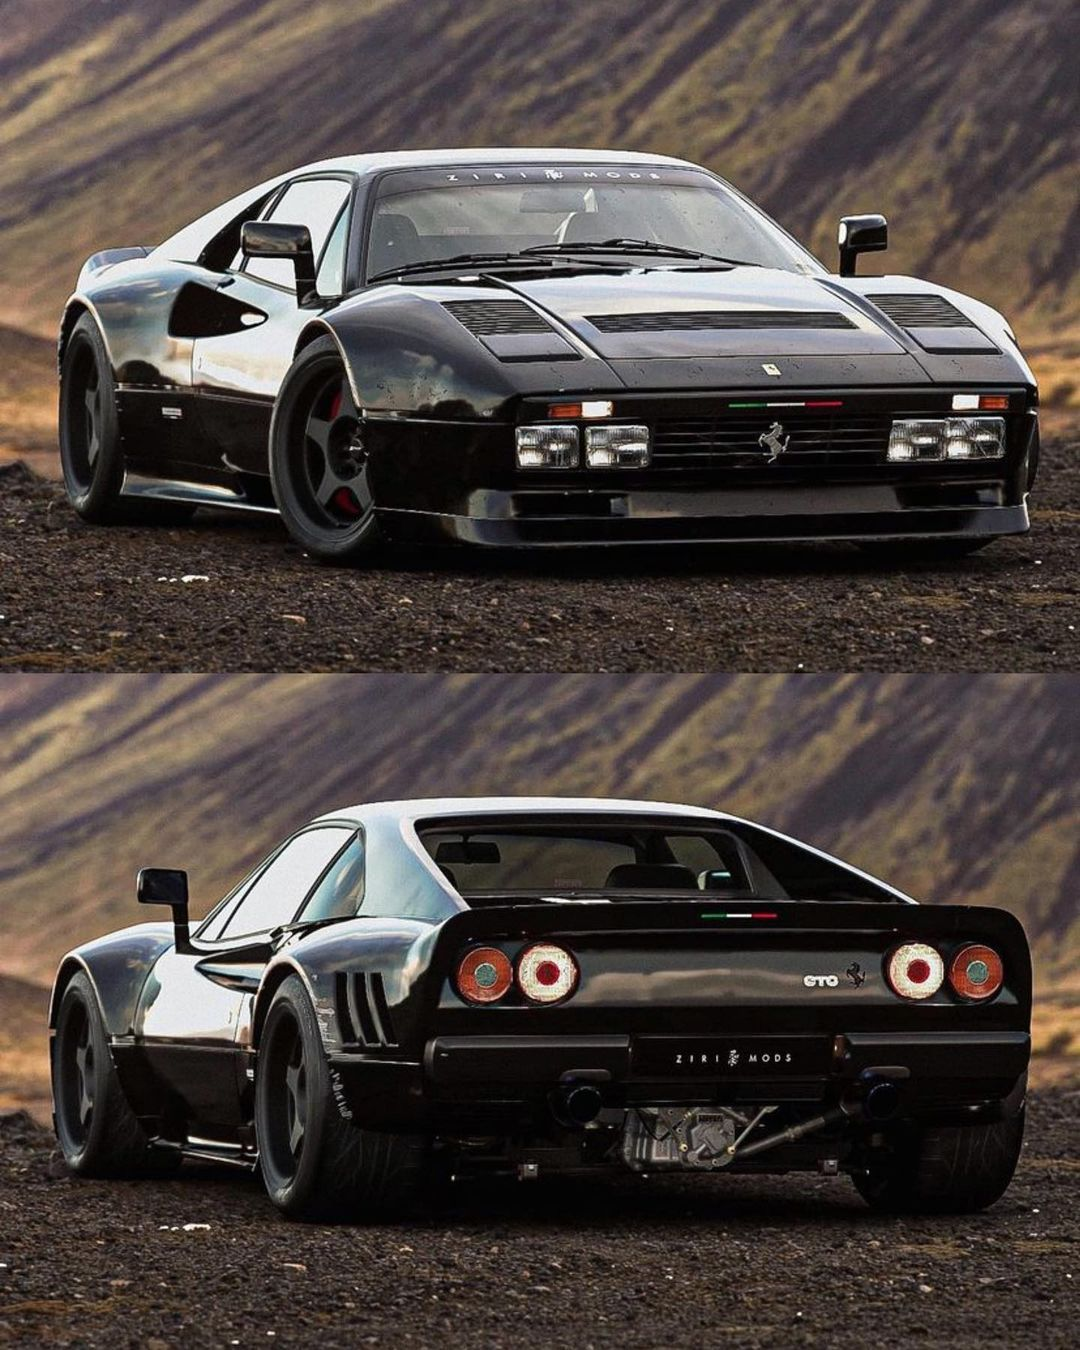
\includegraphics[ width=1.2\textwidth] {Ferrari288GTO.jpg}
\caption{\label{fig:Ferrari288GTO} Ferrari 288 GTO }
\end{figure} 


\begin {enumerate}
\item Topic idea : 
\item Topic idea : 
\end {enumerate}




\begin{equation}
\label {eq:something} 
\min_{x,y} { (1-x)^2 + 100(y-x^2)^2}\\
\end{equation} 

\begin{equation*} % * is without enumeration
\beta_i = 
\frac{\operatorname{Cov} (R_i, R-m)}
	{\operatorname{Var} (R_m)}
\end{equation*} 
In \eqref{eq:something}, we have \ldots


\begin{align*}
(x+1)^3 &= (x+1)(x+1)(x+1) \\
&= (x+1)(x^2 + 2x + 1) \\
&= x^3 + 3x^2 + 3x + 1
\end{align*}

Let X{1}, X{2},...,Xn be a sequence of independant and identically distrubuted random variables with E[X{i}] and 
\begin{equation*}
S{n}=
\frac{1}
	{n}
\sum_{i=1}^{n} X{i}
\end{equation*}


\section {Price}

\begin{tabular}{|l|r|r|} \hline% Argument column specifies column alignment
Item                       & Qty      &     MSRP \$ \\\hline
Ferrari 288 GTO      & 1         &      5     \\\hline

Lamborghini Miura   &2          &      3      \\

Porche 911 GT3       &3          &      2.5    \\\hline
\end{tabular}
\cite{Brooks1997Methodology}
shows that \ldots. Clearly,
all odd numbers are prime
\bibliography{TestReferences}
\bibliographystyle{unsrt}

\end{document}

%Up to typesetting excersise 2